\section{Data Description and Preparation}
\label{sec:data-preparation}

\subsection{Data Description}
\label{sec:data-description}

In this project, we have selected the Global Health Observatory (GHO) data repository under the World Health Organization (WHO) dataset \cite{WHO}.  We considered the data from 2000 to 2015 for 193 countries, in total 2938 rows available for statistical analysis. For each country and year 22 fields are stored. The detailed description of these fileds is presented in table \ref{tab:description}. For our analysis we will use only 2014 year case, so we restricted ourselves to this subset of the original table. It turns out that there are 183 records in the restricted table, which seems to be large enough for the analysis.

\begin{table}
  \centering
  \begin{tabular}{@{}p{0.1\linewidth}  p{0.3\linewidth}p{0.5\linewidth}p{0.1\linewidth}@{}}
    \toprule
      & Column Name     & Description                                                             & type \\
    \midrule 
    1 & Status                 & Developed or Developing status                               & string \\
    2 & Life expectancy   & Life Expectancy in age                                             & float, target variable \\
    3 & Adult Mortality    & Adult Mortality Rates of both sexes (probability of dying between 15 and 60 years per 1000 population) & integer \\
    4 & infant deaths      & Number of Infant Deaths per 1000 population & integer \\
    5 & Alcohol              & Alcohol, recorded per capita (15+) consumption (in litres of pure alcohol) & float \\
    6 & percentage expenditure & Expenditure on health as a percentage of Gross Domestic Product per capita(\%) & float \\
    7 & Hepatitis B & Hepatitis B (HepB) immunization coverage among 1-year-olds (\%) & integer \\
    8 & Measles & number of reported cases per 1000 population & integer \\
    9 & BMI & Average Body Mass Index of entire population & float \\
    10 & under-five deaths & Number of under-five deaths per 1000 population & integer \\
    11 & Polio & Polio (Pol3) immunization coverage among 1-year-olds (\%) & integer \\
    12 & Total expenditure & General government expenditure on health as a percentage of total government expenditure (\%) & float \\
    13 & Diphtheria & Diphtheria tetanus toxoid and pertussis (DTP3) immunization coverage among 1-year-olds (\%) & number \\
    14 & HIV/AIDS & Deaths per 1 000 live births HIV/AIDS (0-4 years) & number \\
    15 & GDP & Gross Domestic Product per capita (in USD) & number \\
    16 & Population & Population of the country & number \\
    17 & thinness 1-19 years & Prevalence of thinness among children and adolescents for Age 10 to 19 (\%) & number \\
    18 & thinness 5-9 years & Prevalence of thinness among children for Age 5 to 9(\%) & number \\
    19 & Income composition of resources & Human Development Index in terms of income composition of resources (index ranging from 0 to 1) & number \\
    20 & Year                     & Year & number \\
    \bottomrule
  \end{tabular}
  \caption{Description of the data set fields}
  \label{tab:description}
\end{table}


As you can see, most of the regressors in the data set are numerical and can be used in the analysis without modifications. There are two regressors, that are not: Status and Country. The first one describes the status of the country and can take two values: ``Developing'' (151 rows) and ``Developed''. This variable was interpreted as factored. As for the second one, country, we decided not to use it in the analysis directly, but, as it will be explained later, it will be helpful to some of the missing values.

\subsection{Missing Data}
\label{sec:missing-data}

In table \ref{tab:missing} we present the information about the missing data in each column of 2014 year data subset. As you can see for almost all of the variables the number of missing data seems to be reasonable. It is not true, unfortunately, for two of them: Population and GDP (i.e. Gross Domestic Product per capita). The number of problematic rows in this case is large, so we should find a way to restore the missing values.

% latex table generated in R 4.0.3 by xtable 1.8-4 package
% Fri Nov 26 11:47:04 2021
\begin{table}[ht]
\centering
\begin{tabular}{rlrrr}
  \toprule
 & name & Present & Missing & MissingPCT \\ 
  \midrule
6 & Population & 142 &  41 &  22 \\ 
  5 & GDP & 155 &  28 &  15 \\ 
  2 & Hepatitis.B & 173 &  10 &   5 \\ 
  9 & Income.composition.of.resources & 173 &  10 &   5 \\ 
  10 & Schooling & 173 &  10 &   5 \\ 
  3 & BMI & 181 &   2 &   1 \\ 
  4 & Total.expenditure & 181 &   2 &   1 \\ 
  7 & thinness..1.19.years & 181 &   2 &   1 \\ 
  8 & thinness.5.9.years & 181 &   2 &   1 \\ 
  1 & Alcohol & 182 &   1 &   0 \\ 
   \bottomrule
\end{tabular}
\caption{Missing data in 2014 year subset}
\label{tab:missing}
\end{table}

Let us consider the Population variable first. It turns out, that for 49 countries for some years data about the population in the WHO table is missing: Cook Islands, Dominica, Marshall Islands, Monaco, Nauru, Niue, Saint Kitts and Nevis, and San Marino have only one missing record each; Eritrea has for misses; and 40 other countries (including USA and Great Britain) do not have any information about the population at all.

It is clear that it is not possible to exclude from the analysis such a large amount of data, so it is highly desirable to find some other source for the missing information. For our future work we selected the table, downloaded from the site \cite{WB}, in which the population for all the years and countries under consideration can be found(in the following it will be referred to as WB table). Some technical work required to import this information into the WHO data set. The reason is the exact spelling of the names of some countries in these two data sets was different. For example, USA in the WHO table was referred to as "United States of America", while in WB table it was named "United States", the other example is "United Kingdom of Great Britain and Northern Ireland" vs simple "United Kingdom".  In total there were 32 such disagreements.

The other important question is what to do with the countries with population data presented both WHO and WB tables, which data source is more reliable? In figure \ref{fig:afghanistan_pop_comparison} Afghanistan population from two data sets is shown. It is clear, that the WHO results does not make any sence: for some years we can observe 2 or 3 order of magnitude leaps. The WB results, on the other hand, are stable, so in the following we will use this table for all countries under consideration.


\begin{figure}
  \centering
  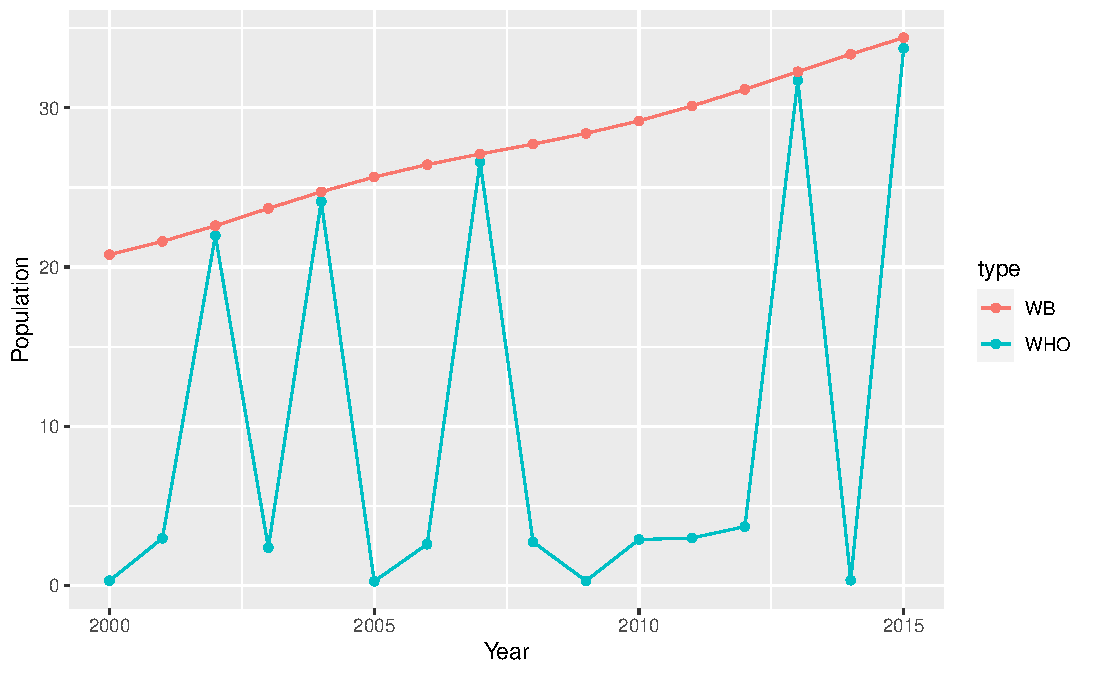
\includegraphics[width = 0.9\textwidth]{figures/Afghanistan_population_comparison}
  \caption{Afghanistan population: comparison of WHO and WB data}
  \label{fig:afghanistan_pop_comparison}
\end{figure}

Almost the same can be said also about the Gross Domestic Product field. For Cook Islands, Monaco, Niue, Papua New Guinea, Saint Kitts and Nevis, San Marino, and Sao Tome and Principe this information is missing in one year; in the case of Eritrea, Iraq, and Libya there are 4 misses per each country; South Sudan and Syrian Arab Republic have 8 misses each and 26 other countries (including UK) do not have any information at all. As a result, for this variable we will be using the data table from Global Health Data Exchange (GHDx) database \cite{GHDx}.

As you can see from table \ref{tab:missing}, in addition to Population and GDP columns, there are also missing values in some other columns, but not a lot. Since data cleaning is not the main part of our project, we decided to simply drop the corresponding rows (only 26 rows were removed) and proceed to the next step.


% \subsection{Variables' Transformation}
% \label{sec:vari-transf}



% ## data description

% ## data cleaning


%%% Local Variables:
%%% TeX-master: "main"
%%% End:
